
\section{Product Line of Product-Line Analyses}


%TODO: Trabalhar na Section 5, formalizando a semântica e colocando uma
%espécie de "cheat sheet" visual: na primeira linha o FM, o workflow, e
%o diagrama; a partir da segunda linha, cada produto da linha indicando
%a expressão de composição que o gera e o desenho correspondente com as
%setas indicando a composição de funções, preservando a localização
%delas em relação ao diagrama original (talvez o diagrama todo possa
%aparecer mais fraquinho ou todo omitido nesse caso; acho que o Revisor
%2 do SCP falou algo do tipo)

%"Next to a strategy, a tiny 'navigation legend' (structure of
%[Fig10]), highlighting the arrows  involved (and eg grayouting or
%removing arrows not involved) would be helpful for a reader, I
%imagine.  If you put a dot in the goal  (Reliability), a 'navigation
%legend' for [Def24] would be down, left  to the dot."


\label{sec:pl2ana}

With the aim of providing a systematic way of using the analysis framework presented in Section~\ref{sec:generalStructure}, 
we define a product line of product-line analysis strategies. By explicitly establishing product line elements, we can guide users in the configuration and instantiation of the framework. 
%Moreover, in Section~\ref{sec:evolpl2ana}, we also explain how this product line evolved.  
%\subsection{Definition of Product Line of Product-Line Analyses}
%\label{sec:defpl2ana}

We use a three-space model~\cite{BorbaPLRefinement} to define the elements from the product line of product-line analysis strategies ($PL^{2}Ana$) as a triplet $(FM,CK,AB)$, where: 

\begin{itemize}
	\item $FM$ is the attribute-based feature model describing the configuration space of product-line analyses, given according to Figure~\ref{fig:fm};
	\item $AB$ comprises the asset base of this product line---in this case, functions and types of the framework in Figure~\ref{fig:strategies-generic};
	% TODO @lmt: we will address the below in the next iteration, right?
	%, as well as formal assets (lemma and theorem statements, and their proofs); 
	\item $CK$ denotes a transformational configuration knowledge~\cite{DOPTransformational} , which maps feature expressions to transformations over AB elements. Intuitively, the CK maps feature expressions to path fragments in the framework.
\end{itemize}


\begin{figure}[t]
	\centering
	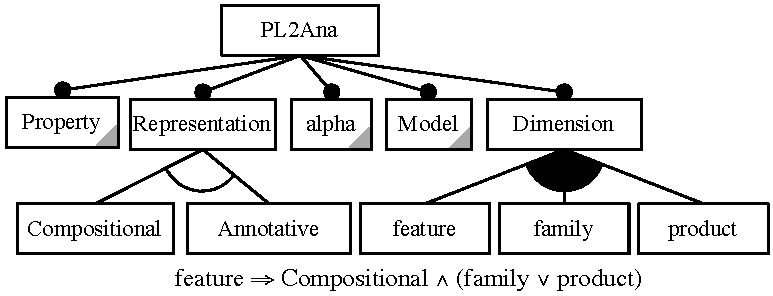
\includegraphics[width = 0.7\linewidth]{figures/fm.pdf}
	\caption{Feature model of the product line of product-line analysis strategies ($PL^{2}Ana$)}
	\label{fig:fm}
\end{figure}
%@TODO lmt: please double check whether "(family or product)" is redundant in the cross-tree constraint.

The feature model shows that $PL^{2}Ana$'s configurability depends on the model and property to be analyzed, on the non-variability analysis function $\alpha$,
on the variability representation (annotative versus compositional), and on dimensions of analysis strategies: feature, family, and product (cf.~\cite{Thum2014}). 
We use the gray triangle in some features to express that we leverage attributes in the feature model to model variability in  property, model, and non-variability analysis function. Attribute values may correspond to the product-line analyses discussed in Section~\ref{sec:strategies} or new analyses on properties allowing an ADD-based representation (cf. Section~\ref{sec:fmkoverview}).  Additionally, the feature model has a cross-tree constraint stating that feature-based analyses require a compositional representation. This way, a configuration of $PL^{2}Ana$ denotes a concrete SPL analysis strategy of a property for a particular model representation.
%specific compositional or annotative representations. 

The asset base comprises foundational elements (types and functions) from which SPL analysis strategies are built as well as their properties. Types refer to models subject to analysis or intermediate analysis results, whereas functions refer to analysis steps. Properties refer to commutative results establishing the soundness of variability-aware 
analyses (cf. Section~\ref{sec:abstraction-description} ). Since the framework targets properties that can be represented in an ADD, as discussed in Section~\ref{sec:fmkoverview}, the functions and types of the lower quadrants of Figure~\ref{fig:strategies-generic}, except \textit{Property}, have the specific interpretation mentioned in Section~\ref{sec:fmkoverview}. However, since we are still interested in an abstract and conceptual description of analyses, the remaining types and functions in $AB$ are either uninterpreted (i.e., we provide no concrete specification nor implementation for them)  or  parameterized, as formalized in Section~\ref{sec:abstraction-description}. For example, the \textit{Product} type is uninterpreted, whereas \textit{Annotative Model} and \textit{Annotative Product Line} are defined directly and indirectly in terms of \textit{Product}, respectively. As additional examples, the $\pi$ function is defined in terms of \textit{Annotative Model} and \textit{Product}; $\alpha$ is uninterpreted, whereas $\hat{\alpha}$ is defined in terms of $\alpha$ and \textit{Annotative Model}.
At a coarse-grained level, all types and functions  must comply with the structure in the diagram. 
%since these also depend on the model and property to be analyzed, \textit{Property}, and $\alpha$ are

The transformational configuration knowledge is responsible for mapping features to transformations over assets. Such transformations are used during product derivation, as explained later in this section. In particular, the model illustrated in Table~\ref{fig:ck} associates feature expressions with type interpretation ($\mathtt{bind}$), partial function application ($\mathtt{select}$), function composition ($\circ$), and function mapping over structure ($\mathit{fmap}$). On the one hand, type interpretation support key concepts in the product-line analysis domain such as $Product$, $Property$, and $\alpha$ to be treated abstractly, thus focusing on its essential concepts and properties, and extending its generality. On the other hand, interpretation needs explicit instantiation, which is a manual step. Partial function application enables selection of the representation of the model to be analyzed: annotative or compositional. The CK additionally uses function composition to combine intermediate analysis steps during product derivation, e.g., 
$\sigma \circ \hat{\alpha}$ combines  the steps of first performing variability-aware analysis ($\hat{\alpha}$) followed by expression evaluation ($\sigma$) when the feature expression $\mathit{annotative} \land \mathit{family} \land \mathit{product}$ in Table~\ref{fig:ck} is satisfied by a configuration. Finally, the CK may also apply analysis steps within a compositional model or expression via $\mathit{fmap}$. For instance, for any configuration of the feature model comprising  the $\mathit{feature}$ feature, the CK applies the variability-aware analysis $\hat{\alpha}$ to all annotative models within the encompassing compositional model.

Additionally, given the cross-tree constraint of the feature model, the compositional representation is also selected, which implies that the type \textit{Compositional Product Line} is instantiated, as specified by the corresponding row in the configuration knowledge. Furthermore, the feature expressions for \textit{Property}, \textit{Model}, and \textit{Representation} evaluate to $\mathtt{true}$, since these are mandatory features, so their corresponding instantiations are always performed. The root feature \textit{PL2Ana} does not appear in the table because it is an abstract feature.



%The transformational configuration knowledge, as stated, is responsible for mapping features into transformations over assets. 
%Since in our case assets are types and functions, the model illustrated in Table~\ref{fig:ck} associates feature expressions with partial function application ($\mathtt{select}$), function composition ($\circ$), and function mapping over structure ($\mathit{fmap}$). 
%Interpretation allows key concepts in the SPL analysis domain such as $Product$,https://www.overleaf.com/project/5dfb7b732691410001bc5ecd $Property$, and $\alpha$ to be treated as parameters of the framework, thus focusing on its essential concepts and properties, and extending its generality. 
%Partial function application enables selection of the concrete model and property to be analyzed, the non-variability aware analysis function, and the representation of the model to be analyzed: annotative or compositional. The CK additionally uses function composition to combine analysis steps, e.g., 
%$\sigma \circ \hat{\alpha}$ combines  the steps of first performing variability-aware analysis ($\hat{\alpha}$) followed by expression evaluation ($\sigma$) when the feature expression $\mathit{annotative} \land \mathit{family} \land \mathit{product}$ holds in Table~\ref{fig:ck}. Finally, the CK  possibly applies these steps in a compositional model or expression ($\mathit{fmap}$). For instance, for a configuration of the feature model comprising both the \textit{feature} and textit{family} features, 
%we compose the corresponding functions in the LHS of Figure~\ref{fig:strategies-generic}. Additionally, given the cross-tree constraint of the feature model, the compositional representation is also selected, which implies that the type \textit{Compositional Product Line} is instantiated, as specified by the corresponding row in the configuration knowledge. Furthermore, the feature expressions for \textit{Property}, \textit{Model}, and \textit{Representation} evaluate to $\mathtt{true}$, since these are mandatory features, so their corresponding instantiations are always performed. The root feature \textit{PL2Ana} does not appear in the table because it is an abstract feature.




%\begin{figure}[t]
%	\centering
%	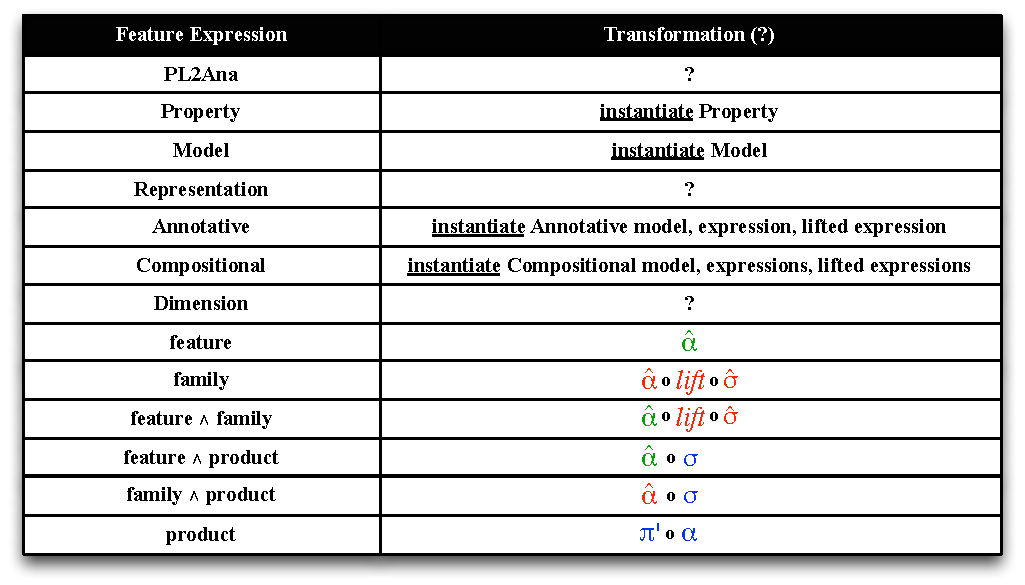
\includegraphics[width = 0.5\linewidth]{figures/ck.pdf}
%	\caption{Configuration Knowledge.}
%	\label{fig:ck}
%\end{figure}

	\begin{table}[htb]
		\centering
		
		\caption{Transformational Configuration Knowledge. Transformation primitives are the functions $\mathtt{bind}$ (type interpretation), $\mathtt{select}$ (partial evaluation), $\circ$ (function composition), and   $\mathit{fmap}$ (mapping over structure). $cModel$ is a compositional model.}
		%\resizebox{\columnwidth}{!}{
			\begin{tabular}{cc}
				\toprule
				
				\textbf{Feature Expression} & \textbf{Transformation} \\\midrule
				$\mathit{Property \mathtt{(true)}}$ & $\mathtt{bind}(\mathit{Property})$  \\
				$\mathit{Model \mathtt{(true)}}$ & $\mathtt{bind}(\mathit{Product})$ \\
				$\mathit{Property} \land \mathit{Model}$     &  $\mathtt{bind}(\mathit{\alpha})$    \\
				%$\mathit{Representation \mathtt{(true)}}$  & $\mathtt{instantiate}(\mathit{Annotative Model})$ \\
				$\mathit{Annotative}$ & $\mathtt{select}(\mathit{Annotative Product Line})$ \\
				$\mathit{Compositional}$  & $\mathtt{select}(\mathit{Compositional Product Line})$ \\    
				$\mathit{annotative} \land \mathit{product}$   &  $  \alpha  \circ \pi  $  \\    
				$\mathit{compositional} \land \mathit{product}$  &  $  \alpha \circ \pi' $  \\    
				%$\mathit{family} \lor \mathit{feature}$  & $\mathtt{instantiate}(\mathit{\hat{\alpha}})$  \\    
				$\mathit{annotative} \land \mathit{family} \land \mathit{product}$ &  $\sigma \circ \hat{\alpha}$  \\    
				$\mathit{annotative} \land \mathit{family}$ &  $\hat{\sigma}  \circ \mathit{lift}   \circ \hat{\alpha} $  \\    
				$\mathit{feature} \land \mathit{product}$  & $  \sigma  \circ \mathit{fmap(\hat{\alpha})} $ \\    
				$\mathit{feature} \land \mathit{family}$  & $ \hat{\sigma} \circ \mathit{fmap(lift)} \circ \mathit{fmap(\hat{\alpha},cModel)}$ \\    
				%$\mathit{product}$    &  $\mathtt{instantiate}(\mathit{\alpha})$    \\    
				\bottomrule
			\end{tabular}
		%}
		\label{fig:ck}
	\end{table}





$PL^{2}Ana$'s products are then product-line analysis strategies for a given model, property, and an originally non-variability-aware analysis technique. Figure~\ref{fig:ad} describes $PL^{2}Ana$'s product derivation process. First, one manually binds--or reuses previously specified--the model, the property to be analyzed, and  the non-variability aware analysis. Following, one decides on the representation (annotative versus compositional). Finally, one chooses the analysis dimensions (feature, family, product). 
Derivation then proceeds by evaluating the $CK$ according to the given configuration, progressively composing the intermediate results of transformations of AB elements corresponding to feature expressions satisfied by the product configuration at hand. Therefore, the resulting product is a specific product-line analysis strategy corresponding to an analysis path in the framework represented in Figure~\ref{fig:strategies-generic}. This product  is build by reuse of AB elements and corresponds to a concrete PVS theory comprising exactly the corresponding analysis function, supporting types, and properties.

% \begin{figure}[t]
% 	\centering
% 	\resizebox{\textwidth}{!}{%
% 	    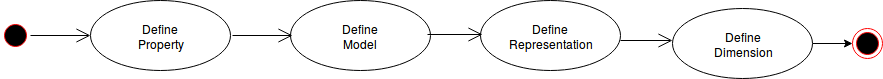
\includegraphics{figures/ad.tikz}
%     }
% 	\caption{Product Derivation Workflow}
% 	\label{fig:ad}
% \end{figure}
% %@TODO: update figure to insert taks "Define alpha (non-variability analysis) after "Define Model"

\begin{figure}[t]
	\centering
	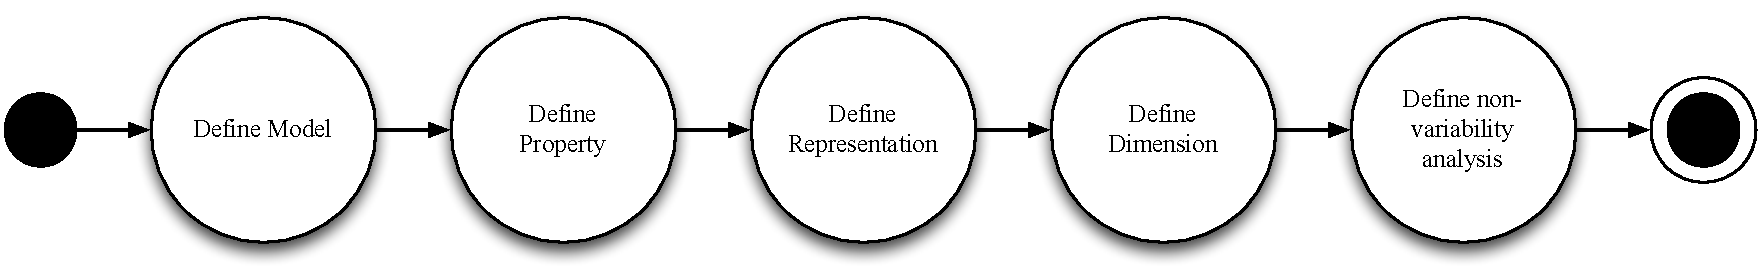
\includegraphics[width = 0.9\linewidth]{figures/workflow.pdf}
	\caption{$PL^{2}Ana$'s product derivation process}
	\label{fig:ad}
\end{figure}

An example of $PL^{2}Ana$'s product derivation process is given in Figure~\ref{fig:workflow-reliability}. 
We see that we might derive a family-product reliability analysis for annotative models 
by binding property and model attributes as Reliability and DTMC, respectively. 
Moreover, we select the representation and analysis dimension accordingly, 
to produce an analysis strategy that corresponds to the top-right quadrant of Figure~\ref{fig:strategies-generic}, 
particularly instantiated with the chosen property and model. 

\begin{figure}[htbp]
	\centering
	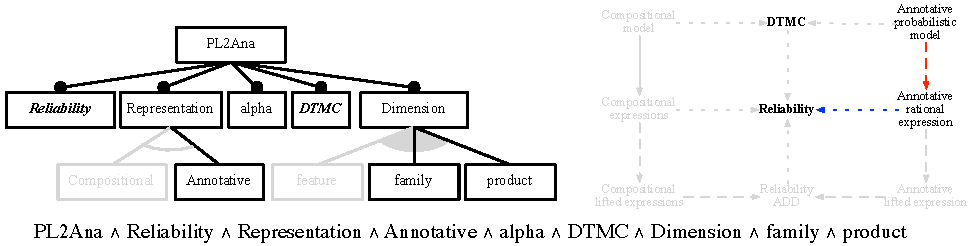
\includegraphics[width=0.9\linewidth]{figures/workflow-reliability.pdf}
	\caption{Example of $PL^{2}Ana$'s product derivation process with reliability analysis}
	\label{fig:workflow-reliability}
\end{figure}

Another example of $PL^{2}Ana$'s product derivation process is given in Figure~\ref{fig:workflow-behavior}. In this example, we derive a feature-family behavior analysis for compositional models (SMV and fSMV)
by choosing CTL and TS as property and model attributes, respectively. 
Moreover, we select the representation and analysis dimension accordingly, 
to produce an analysis strategy that corresponds to the LHS of Figure~\ref{fig:strategies-generic}, 
particularly instantiated with the chosen property and model. We note that this instance extends the scope of the state-of-the-art of product-line behavior analyses represented in Figure~\ref{fig:diagram-FTS}, thereby providing evidence that the configurability of our framework allows exploring novel analyses.

\begin{figure}[htbp]
	\centering
	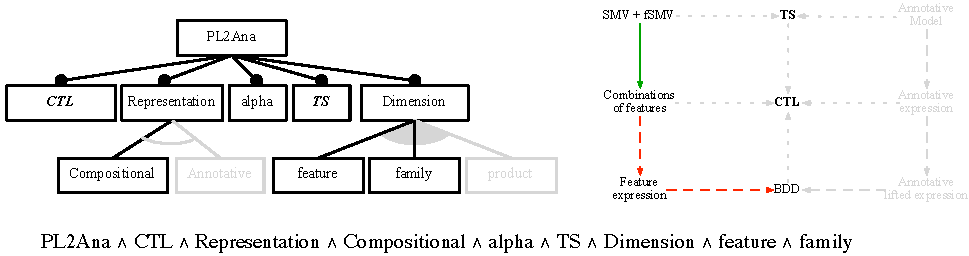
\includegraphics[width=0.9\linewidth]{figures/workflow-behavior.pdf}
	\caption{Example of $PL^{2}Ana$'s product derivation process with behavioral analysis}
	\label{fig:workflow-behavior}
\end{figure}


%vra: I think we should consider dropping this section, since it looks outside the main focus
%\subsection{Evolution of Product Line of Product-Line Analyses}
%\label{sec:evolpl2ana}
%In Section~\ref{sec:abstraction-description}, we addressed the generalization of the the analyses represented in Figure~\ref{fig:strategies-overview}. Essentially, we abstracted fundamental concepts (property, model, non-variability-aware analysis) into uninterpreted types and dependent concepts into parametrized types and functions  with assumptions along the structure of the diagram. In this section, we describe the development of product lines of product-line analyses in terms of a principled evolution of previous works. Such evolution can be useful for further safe evolution of the proposed framework.

%Motivated by the need to empirically compare the proposed feature-family reliability analysis strategy to other strategies, \citet{LANNA2017} implemented the ReAna tool, which actually realizes the diagram in Figure~\ref{fig:strategies-overview}. 
%As depicted in Figure~\ref{fig:evol}, such evolution can be safely described by applying  the \textit{merge template}~\cite{NevesBATTSK15} to incrementally evolve the product line, starting from the feature-family-based~\cite{LANNA2017} and feature-product-based strategies~\cite{Ghezzi2013}, then incorporating the family-product-based~\cite{nunes_variability_2012} and lastly the family-based~\cite{FDTMC}  strategies. The process' soundness  follows from the soundness of the employed template. 

%\begin{figure}[t]
%	\centering
%	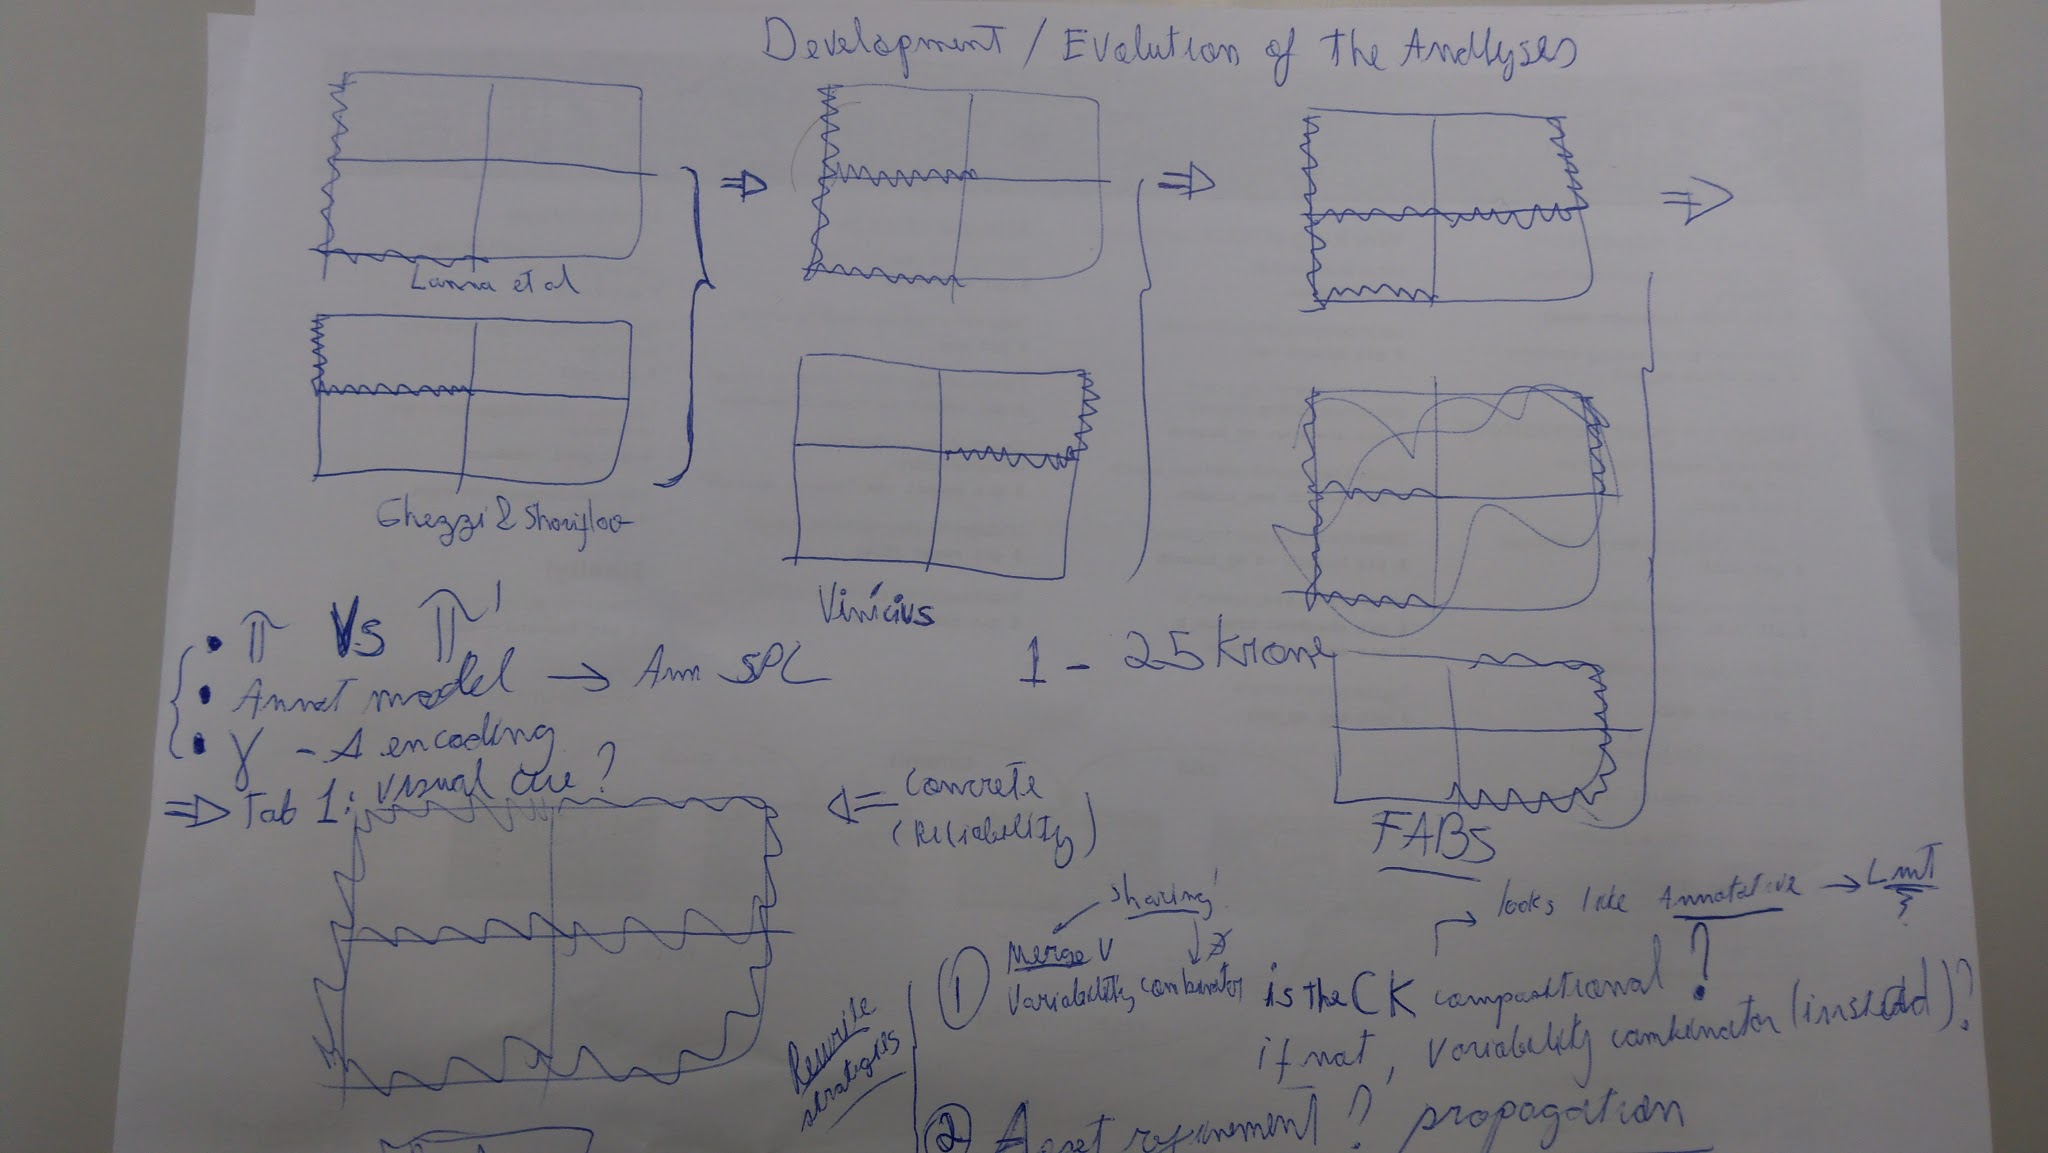
\includegraphics[width = 0.9\linewidth]{figures/evol.jpg}
%	\caption{Evolution of Product Line of Product-Line Reliability Analysis Strategies.}
%	\label{fig:evol}
%\end{figure}



